\chapter{Background}\label{ch:baseline}%

\section{Goal-oriented Requirements Engineering}

Goal-oriented requirements engineering (GORE) captures the intentionality behind system requirements. More than just presenting the \textit{what} and the \textit{how} of a system-to-be, it provides the reasoning for each requirement, that is, they also present the \textit{why}. Through a directed graph tree that begins with a root goal, goals are connected through decomposition links. Root and higher level goals are related to strategical concerns, while lower level and leaf-goals are related to technical and operational features of the system. 

The main purpose of a goal model is to support the early process of RE, including the elicitation of social needs and dependencies, the actors involved in delivering functionalities and resources, the decomposition of higher-level goals into more granular and detailed requirements chunks, the operationalization through means-end tasks and finally the comparison between different alternatives for the system-to-be. A goal model is said to be valid and complete if it follows all its syntactic rules and if all system goals are either decomposed, delegated to other actors or fulfilled by operational system tasks. 

Frameworks and methodologies like the i*~\cite{Yu1996}, KAOS~\cite{Dardenne1993} and TROPOS~\cite{Bresciani:2004} represent the foundations for the goal model analysis used by a variety of other proposals. Despite some syntax differences, most goal-oriented approaches share a set of common and core important concepts:
\bigskip

%\Large{\underline{Intentional entities}}
%\normalsize

\subsection{Intentional Entities}

\begin{itemize}

\item \textbf{Actor:} an entity that has goals and can decide autonomously how to achieve them. They represent a physical, social or software agent. For example: a patient, an emergency center, a doctor and a Mobile Personal Emergency System running in patient's smartphone.
\medskip

\item \textbf{Goal:} actors' strategic interest. A goal with a clear-cut criteria for its satisfaction is called a hard goal. In opposition, softgoals have no clear-cut criteria for deciding whether they are satisfied or not and usually represent non-functional requirements. For example: vital signs are monitored, emergency is detected, emergency center is notified (hard goals) and emergency awareness, precise assistance, feel supported (softgoals).
\medskip

\item \textbf{Task:} an operational means to satisfy actors' goals. For example: monitor temperature sensor, persist vital signs data, request emergency assistance.
\medskip

\item \textbf{Resource:} an information data or a physical resource that is generated or required by an actor. For example: a form input from the user, an exported file, the power from the battery component, etc.

\end{itemize}

%\Large{\underline{Relations}}
%\normalsize

\subsection{Relations}

\begin{itemize}

\item \textbf{AND/OR Decomposition:} AND-decomposition (OR-decomposition) is a link that decomposes an actor's goal/task into actor's sub-goals/tasks, meaning that all (at least one) decomposed goals/tasks must be fulfilled/executed in order to satisfy its parent entity. 
\medskip

\item \textbf{Means-end:} a relation that indicates a means to fulfil an actor's goal through the execution of an operational task by the same actor.
\medskip

\item \textbf{Contribution link:} a positive or negative contribution between a given goal/task to a softgoal. Contribution links are used for deciding between alternative goals/tasks at design time (contribution analysis).
\medskip

\item \textbf{Dependency link:} a delegation of a goal, task or resource (\textit{dependum}) from an actor (depender) to another (dependee).

\end{itemize}

\section{TROPOS Methodology}

TROPOS is a GORE methodology based on the i* framework~\cite{Bresciani:2004}. Its main improvement to the i* framework is the addition of new phases of requirements engineering, architecture and system design, namely:

\begin{itemize}

\item Late requirements engineering: Beyond the social dependency modelling with actors diagrams representing stakeholders and their needs in early requirements phase, a late requirements phase focuses on the system actor analysis. In this phase, system goals are inherited from stakeholders needs and represent both functional and non-functional requirements. Each goal has to be further decomposed in more granular sub-goals, delegated to other actors or to be fulfilled by means-end tasks. 
\medskip

\item Architectural design: In this phase, new actors representing sub-systems are created to fulfil different system goals. The idea is to shape the solution using a multi-agent architecture style instead of a monolithic system approach. Data and control interconnections are represented as dependencies.
\medskip

\item Detailed design: The last phase is characterized by the specification of agent capabilities and interactions though UML activity and sequence diagrams. Also, the implementation platform and other specific implementation details are addressed in order to directly map the design to system code.

\end{itemize}

%TROPOS implementation phase is out of the scope of this work as our objective is to improve the analysis and the solution that will be later implemented.

\section{Goals, Means and Contexts}

Context may be defined as the reification of the environment that surrounds the system operation~\cite{Andrea01aframework}. Contexts, as already stated, may not be static, but dynamic, and a system has no control over the context variation. Accordingly, a system must be able to support different contexts of operation without violating its functional and non-functional goals. To achieve this, systems must be able to monitor the state of their surrounding environment and take adaptive actions regarding the alternatives used for fulfilling their goals.

%decide which alternative will be used regarding both the availability of that alternative and the optimization of non-functional requirements.

In a contextual goal model (CGM), dynamic contexts may affect what goals a system have to reach, the means available to meet them and also the quality achieved by each alternative~\cite{Ali:2010}. Root goals and higher-level strategical goals are generally not contextualized as they represent the main purpose of a system~\cite{Andrea01aframework}. As these goals are decomposed in more granular sub-goals, a context condition may affect:

\begin{enumerate}

\item If one or more goals are required for that context, limiting \textit{what} a system should do. For instance, the goal `track person's location' is only required in the context `patient is not at home'.
\medskip

\item If a sub-goal or task is adoptable, limiting the `means' to fulfil a required goal. For instance, `track by GPS' may not be used in the context `battery is low' (stakeholder preference) or `no GPS signal' (technical impediment).
\medskip

\item The positive, neutral or negative contribution of one alternative to a qualitative softgoal or to a non-functional metric. For instance, the precision of each geolocation method - voice call, mobile triangulation and GPS variate according to contexts like the health condition of the person and the strength of mobile and GPS signals.

\end{enumerate}

Context effects may have different causes, among them:

\begin{itemize}

\item \textbf{Stakeholders preferences:} At a certain context, a stakeholder need (dependency) that justifies a system goal may cease to exist (goal restriction); or it may prefer a given alternative to another (means restriction). %usually because in this context he/she/it finds it to be more.
\medskip

\item \textbf{Technical impediments:} At a certain context, a required information or physical resource may not be available, imposing a restriction on the selection of one or more alternatives (means restriction).

\end{itemize}

%The third effect is the main focus of this work, as it is related to non-functional requirements such as dependability attributes. Also, the other effects must also be considered by the verification model, including the variability at what goals are required at each context and what means are adoptable, resulting in a more realistic and precise verification of corresponding metrics.

%the GORE contribution analysis that we aim to improve. In our proposal, we extend the concept of the context variation effect to non-functional metrics of goals and tasks - as the components used for concrete task execution may also be affected by context variations, e.g., the reliability of a sensor in different temperatures. 

\section{Variability in GORE}\label{sec:variability}

Given the possibility of an OR-decomposition in a goal model, more than one alternative can exist in terms of which subgoal should be achieved to satisfy its upper goal,  which subtask should be executed to satisfy its upper task or which task should be executed to satisfy its upper goal. Accordingly, multiple paths may lead to the satisfaction of the root goal. They are called alternative behaviours, or alternatives. Solving the variability problem in goal models has different meanings according to the development phase it takes place. 

\subsection{Design-time analysis}

At design time, multiple alternatives are elicited through goal-oriented analysis, but not all are selected to be part of the system-to-be. In traditional GORE, contribution analysis is used for the comparison of how each alternative contributes for one or more softgoals. Usually, only one alternative with the more positive contribution sum is selected for the system-to-be. Or, as in the simplistic example of Figure~\ref{fig:GORE_CA}, the decision relies on the softgoals priorities~\cite{Yu:2013}.

\begin{figure*}[h!]
\centering
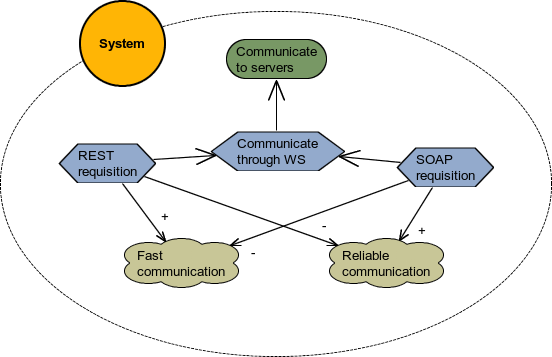
\includegraphics[width=0.6\textwidth]{imgs/GORE_CA.png}
\caption{Contribution analysis in TROPOS GORE.}
\label{fig:GORE_CA}
\end{figure*}

\subsection{Runtime analysis}

In contrast to the design-time variability in goal models, runtime variability depends on runtime input and must be preserved at runtime, i.e., variability is inherited by the solution design~\cite{Yu:2008}. A runtime analysis should select the valid alternative according to stakeholders preferences and the current context of operation.

The contextual goal model tackles the influence of the context on the autonomous decision of which alternative should be selected~\cite{Ali:2010}. For instance, if the monitored traffic condition is `jammed' and the patient's condition is `critical', an emergency chopper is selected for assistance in the place of an ambulance. We call this  `direct context implication'.

In other cases, alternatives should be monitored and analysed in terms of non-functional metrics to decide which one is suitable or for selection. Here, the context of operation does not directly defines the adoptable alternative, but its effect on the quality of each alternative is considered as a decision criteria. For instance, a more complex analysis must estimate the probability of the ambulance to reach the patient in less than X time units given a traffic condition. We call this `indirect context implication'. 

%Both cases - the direct and indirect context effect over the selection - may integrate the analysis of a self-adaptation feedback loop.

\begin{figure*}[h!]
\centering
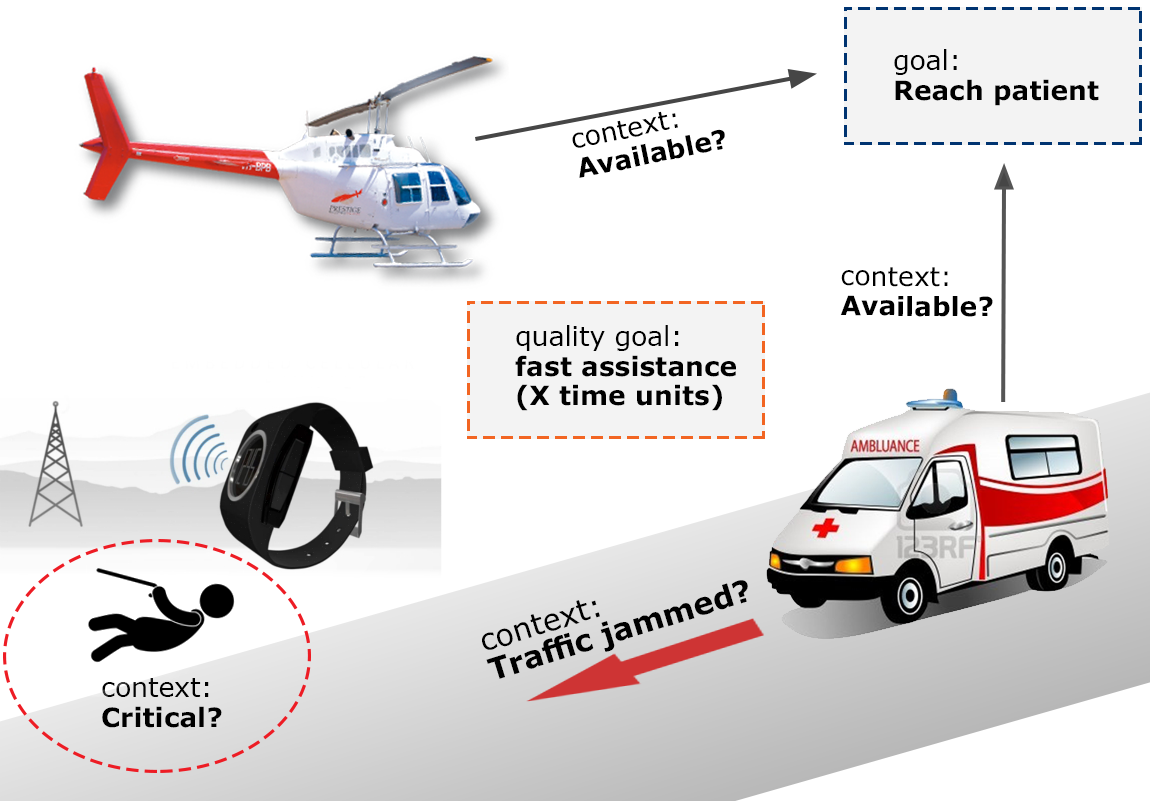
\includegraphics[width=1\textwidth]{imgs/RUNTIME_ANALYSIS.png}
\caption{Contribution analysis in TROPOS GORE.}
\label{fig:RUNTIME_ANALYSIS}
\end{figure*}

In Figure~\ref{fig:RUNTIME_ANALYSIS}, the availability of the emergency resources are contexts that directly restricts the adoption of corresponding means to reach a patient. In contrast, the traffic condition affects the time to reach the patient, i.e., this context indirectly affects the selection of an ambulance and requires further analysis to estimate the assistance time in different traffic conditions. Also, the context `patient health' affects the time restriction in the `fast assistance' quality goal. This scenario leads to the following question: Among the available functional alternatives, which also fulfils the quality goal in the current context?


%Our proposal aims to solve the variability in goal models at runtime through a probabilistic verification of system alternatives in multiple contexts of operation following both direct and indirect context effects over alternatives.

%to select the best alternative at design time for the system-to-be, or to select the best alternative at runtime for the system in operation. Both problems are related to how each alternative conforms to requirements in terms of softgoals and non-functional metrics and to the context of operation. At design time, estimation of NFR is conduced on the model of the system behaviour. 

%\subsection{Different paths, one context, one solution}
%
%Despite the elicitation of more than one path, only one alternative is kept at design time. Softgoals are generally used as criteria for the alternative selection~[i*, TROPOS, KAOS]. We extend TROPOS with a model-based verification of  non-functional constraints. Verification should point out at design time:
%
%\begin{enumerate}
%
%\item Which alternative conforms to the non-functional metrics associated to the goal model. 
%\medskip
%
%\item The best alternative given one or more metrics. In the last case, a multi-criteria approach should decide which alternative will be selected for the system-to-be.
%
%\end{enumerate}
%
%\subsection{Different paths, multiple contexts, multiple  solutions}
%
%A system affected by context variation may have to select different alternatives for different contexts, justifying variability in the system-to-be design. Solving variability becomes more complex as for each context a different alternative may provide the best contribution to softgoals and achieve higher values for non-functional metrics. 
%
%In our work, variability solving for multiple contexts involves an iterative verification in which contexts are analysed for all adoptable alternatives. At least one alternative must be able to fully satisfy both functional and non-functional requirements of the system.

%The later corresponds to the family verification of a dynamic software product lines~[GENAINA].

\section{Dependability}

The concept of dependability is related to dependence and trust as well as to the ability of a system to avoid failures that are more frequent and more severe than certain threshold~\cite{Laprie2004}. According to Avizienis et al., dependability encompasses the following attributes: 

\begin{itemize}

\item Availability: readiness for correct service.
\medskip

\item Reliability: continuity of correct service.
\medskip

\item Integrity: absence of improper system alterations.
\medskip

\item Safety: absence of catastrophic consequences on the user(s) and the environment.
\medskip

\item Maintainability: ability to undergo modifications and repairs.
\medskip

\end{itemize}

%Correctness is opposed to failures. 

%MAY BE USEFULL IN OTHER SECTION
%A holistic dependability specification has to include not only the software operation, but also the NFRs for which that operation is meant. Non-functional requirements are an important factor to decide the acceptable frequency and severity of a software or hardware failure.

A failure is a perceived deviation from system expected behaviour that may have variable degrees of consequence on the user(s) and the environment. These failures are caused by specification faults or specification violations. In the first case, requirements and behaviour models fails to describe the system: either the goals or the means to fulfil then are incorrect, inappropriate or incomplete. In the second case, software or hardware behaviour did not follow its specification due to a natural phenomena, a human-made fault, a malicious fault or an interaction fault~\cite{Laprie2004}.

Avezienis et al. distinguishes faults from errors and failures in a fault causality chain. In their definition, errors are part of the system's total state that may lead to failures. Failures are characterized by deviations in the external service state, i.e., by external errors. In turn, errors are caused by faults, resulting in the following chain: $$ fault \rightarrow error \rightarrow failure$$ 

In most cases, a  fault first causes an error in an internal state of a system. Not all internal deviations results in external deviations, i.e., not all internal errors result in failures. External faults may also result in internal errors and possibly subsequent service failure(s), but only if a prior vulnerability exists, i.e., a previous internal fault enabling the external fault to harm the system. 

Failures can be characterized by different viewpoints. In this work, one important aspect is the failure consequence level, as it describes the consequence of failures to user(s) and to the environment. Two limiting levels are defined by Avezienis et al.:

\begin{itemize}

\item \textbf{Minor consequence:} where the harm caused by a failure is not higher than the benefit of the correct system behaviour. For instance, a momentary interruption in a video streaming service.
\medskip

\item \textbf{Major consequence:} where the failure harm is incommensurable higher than the benefit of the correct service. For example, the death of a user.
\medskip

\end{itemize}

Other intermediary levels may exist according to each case. In a goal model, the consequence level viewpoint may characterize the failure in achieving one or more system goals. For instance, a failure in fulfilling a goal with higher relevance in the goal tree of a critical system would have a catastrophic consequence. There are many means to attain systems dependability. Avezienis et al. groups them in four major categories:

\begin{itemize}

\item \textbf{Fault prevention:} means to prevent the occurrence or introduction of faults. 
\medskip

\item \textbf{Fault tolerance:} means to avoid service failures as a consequence of faults.
\medskip

\item \textbf{Fault removal:} means to reduce the number and severity of faults.
\medskip

\item \textbf{Fault forecasting:} means to estimate the present number, the future incidence, and the likely consequence of faults.

\end{itemize}

The scope of this work is restricted to specification violations, i.e., we assume that a system specification is complete and consistent. Failures are caused by anomalous behaviour of the components participating in the execution of system tasks, including technical components and human actors. Regarding the different means to attain dependability, our goal-oriented dependability analysis is classified as a fault forecasting, as it aims to estimate the probability of different system goals in being fulfilled.

% and consequently to the tasks responsible for their fulfilment. 

%PROPOSAL
%Depending on how a goal is decomposed until they are ultimately satisfied by tasks, a task failure may or may not implicate in a goal failure. A goal-oriented failure forecasting as part of a dependability analysis must take into consideration the combination of the original goal model rationale the behaviour specification of a RGM - for instance, in OR-decomposition of multiple tasks, the success of one task is enough for the goal satisfaction.

%The relation among faults, errors and failures is called fault causality chain.


%Avizienis et al. also characterizes a failure according to four viewpoints. For this work, failure domain and failure consequence are important as they define .



\section{Probabilistic Model Checking}

% Also, some algorithms are designed to generate random outputs. 

Many systems are susceptible to various phenomena of stochastic nature and to non determinism in their behaviour. For example, failures may be caused by unpredictable events and by unreliable components. In contrast to model checking techniques for which the absolute correctness of a system is verified, a probabilistic model checking aims to verify properties over transitions systems enriched with probabilities~\cite{Baier:2008}. Accordingly, PMC allows quantitative statements to be made about the system's behaviour, expressed as probabilities or expectations, in addition to the qualitative statements made by conventional model checking~\cite{Kwiatkowska:2012}.

Among the most popular types of transition systems employed in PMC are those based on Markov chains, e.g., the discrete-time Markov chain (DTMC) and the Markov decision process (MDP)~\cite{Kwiatkowska:2012}. Also, probabilistic operators extends the conventional time-bounded or unbounded temporal logics for property specification. Regarding dependability, the PMC technique enables the forecasting of system performance and dependability based on probabilistic events and behaviour described in probabilistic models. As a model checking technique, PMC requires:

\begin{enumerate}

\item a description of the system to be analysed, typically given in some high-level modelling language, e.g., in PRISM language.
\medskip

\item a formal specification of quantitative properties of the system that are to be analysed, usually expressed in variants of temporal logic, e.g., in PCTL.
\medskip

\end{enumerate}

In PMC, the system description is converted to a probabilistic model. In addition to the quantitative information regarding the probability and/or timing of the transition's occurrence, Markov chains can also be augmented with \textit{rewards} used to specify additional quantitative measures of interest~\cite{Kwiatkowska:2009}. In future works, the reward structure could be useful for extending our goal-oriented dependability analysis with the verification of restricted resources consumption like the battery energy.

%A model checking is a formal method that aims to automatically verify the correctness of a system model. Probabilistic model checking supports the verification of finite-state probabilistic models such as discrete-time Markov chain (DTMC), continuous-time Markov chain (CTMC) and Markov decision process (MDP). Different types of properties enables the verification of a vast range of non-functional metrics.

\subsection{PRISM tool}

%PRISM allows the modelling and analysis of systems which exhibit random or probabilistic behaviour. 

The PMC technique used in this approach is supported by the PRISM probabilistic model checker tool~\cite{PRISM:main}. The decision of using PRISM as the probabilistic state-based model checker was due to the richness of its environment and to the number of successful case studies that have used this tool, indicating its maturity~\cite{PRISM:pubs}.

%, and also due to its rich environment that is able to represent different kinds of probabilistic models and their evaluations. 

PRISM is suitable for different kinds of model evaluations depending on the abstraction level, the type of probabilistic model and the PCTL properties to be analysed. Both qualitative and quantitative analysis are available features in the simulation/verification environment. Other environments for modelling and property specification are also available in the tool.
  
\subsection{PRISM language}

PRISM language~\cite{PRISM:language} offers a rich set of constructs that may represent system modules, components and others architectural and design abstractions. Modules are the main structure in a PRISM model. They are composed of variables and commands. The first describes the finite states a module can be in. The later describes the behaviour of a module, i.e., the actions that may result in state transitions and are guarded by predicates which in turn can be composed of any variable in the model. Finally, labels are used for command naming and synchronization. A DTMC command in PRISM takes the following form: $$[action]<guard>\to<probability>:<update>;$$

\subsection{Probabilistic Computation Tree Logic}

PCTL is a temporal logic based on the Computation Tree Logic (CTL). Its main difference from CTL is the probabilistic operator $ P_J(\varphi)$, where $\varphi$ is a path formula and $J$ an interval in [0,1] indicating a lower and/or upper bound on the probability. $ P_J(\varphi)$ may be read as the probability of a set of paths satisfying $\varphi$ and starting at state $s$ to meet the bounds given by $J$~\cite{Baier:2008}.

%Path formula \varphi definition is similar to CTL, except that a bounded until operator is additionally incorporated to specify that a path formula . 

The specification of domain-specific dependability properties with PCTL has been explored in previous works~\cite{Kwiatkowska:2009, Nunes:2012, Kwiatkowska:2012}. For example, the reachability property expressed by formula $P=?\ [\ F\ (\varphi)\ ] $ computes the probability that a system will eventually reach a state that satisfies $ \varphi $. Accordingly, the satisfaction of this formula guarantees that a final successful system state will be reached regardless of the time elapsed to reach it. A time-bounded variant would express a similar event in a restricted number of transitions or time units. 

In our proposal, PCTL formulas may be specified to verify different properties of a runtime goal model mapped to a DTMC verification model. In specific, our goal-oriented dependability analysis focus in the time-unbounded reachability of the states representing the fulfilment of one or more system goals.

\subsection{PARAM}

The powerful analysis environment offered by PRISM tool is limited by the verification of a single combination of initialized variables at a time. For instance, if a variable represents the probability of a transition in the model, PRISM requires the initialization of this value to produce a fixed output for a given specified property. At most, PRISM allows the creation of experiments with undefined variables ranging from two limits at a fixed step value. 

A parametric model checking provides a more flexible analysis, as constant variables in the model can be replaced by parameters~\cite{Hahn:2010}. Regarding the PMC, the PARAM tool extends the PRISM language with the additional reserved word \textit{param} to be used with variables describing state transition probabilities. Given a probabilistic model with additional param variables and a PCTL property, a corresponding parametric formula is generated.

The main benefit of the parametric formula generated by PARAM is to enable the verification of multiple combinations of values for each parameter in an efficient manner, as the probabilistic model checking problem has been previously solved by the tool. Also, different sorts of postprocessing operations can be performed by computer algebra packages, e.g., to find the optimal parameter settings and to evaluate the parametric formula for a given setting~\cite{Hahn:2010}.

In our proposal, a parametric formula generated offline could be evaluated at runtime analysis and integrate a self-adaptation loop. The formula scalability is a relevant concern, as previous works have demonstrated its exponential relation with the number of parameters in the model~\cite{VINICIUS}. Nonetheless, depending on the modelling approach and the scope of the verification, parametric model checking can be proven an efficient approach for dependability analysis. The scalability of our goal-oriented dependability analysis based on probabilistic PMC is addressed by our fourth research question.

More recent PRISM versions also supports a parametric model checking. Nonetheless, PARAM has been successfully evaluated in more case studies in which it has been proved a reliable and stable tool, justifying its adoption by this work in detriment of the built-in PRISM parametric analysis. 

%In this work, PARAM has been used for the generation of parametric formulas as part of the goal-oriented dependability analysis. 

%\subsection{Dependability analysis with PMC}
%
%
%
%%As it will be explained in later sections, goal models may be extended with the behaviour specification required for the verification of some important dependability attributes. The objective is to anticipate non-functional dependability violations and to support the decision of which alternatives to use at runtime self-adaptation. 
%
%A model checking technique should be used for dependability analysis as long as: 
%
%\begin{itemize}
%
%\item A formal system model may be built;
%\medskip
%
%\item Properties representing dependability attributes may be defined;
%\medskip
%
%\item The analysis overhead is justified, e.g., by its criticality.
%\bigskip
%
%\end{itemize}

%That is, instead of providing the final evaluation for a given property, models may use parameters instead of initialized variables and the verification will output a parametric formula whose evaluation will estimate or verify the model for any valid combination of parameters values.

\section{Antlr Language Recognition Tool}

ANTLR (Another Tool for Language Recognition) is a open source parser generator for reading, processing, executing or translating structured text or binary files~\cite{Parr:2007}. The main purpose is to automatically generate a parser for a custom language defined in a specific grammar supported by the tool. The parser can then be imported by any JAVA compatible project to build and walk parsed trees from an input stream. 

As a result, domain-specific languages may parsed using JAVA methods that will manipulate primitive attributes and objects according to what each parser rule and lexical term means for that language. In our proposal, ANTLR was successfully used to generate the parser for the regular expression language that specifies the behaviour in a runtime goal model and for the context effect notations as proposed by the contextual goal model. Listing~\ref{lst:ANTLR_GRAMMAR} presents the grammar used in the RGM parser. Further details for both parser rules and lexical terms is given in later section.

\begin{lstlisting}[style=ANTLR, caption={ANTLR grammar for the RGM behaviour regex},label={lst:ANTLR_GRAMMAR}] 
grammar RTRegex;
rt:     expr NEWLINE				# printExpr
  |     NEWLINE					# blank
  ;

expr:   expr op=`+' expr			# gCard
    |	expr op=`|' expr			# gAlt
    |	`opt(' expr `)'				# gOpt
    |   `try(' expr `)' '?' expr `:' expr       # gTry
    |	expr op=(`;'|`#') expr			# gTime
    |   SKIP					# gSkip
    |   GID                                     # gId
    |   FLOAT					# n
    |   `(' expr `)'                            # parens
    ;

GID     	: [GT] FLOAT		;
FLOAT		: DIGIT+`.'?DIGIT* 	;
SEQ             : `;'			;
PAR             : `#'			;
ALT		: `|'			;
SKIP		: `skip'		;
NEWLINE : [\r\n]+               	;
WS              : [\t]+ -> skip 	;

fragment
DIGIT		: [0-9]			;

\end{lstlisting}